\documentclass[10pt,landscape]{article}

\usepackage{multicol}
\usepackage{calc}
\usepackage{ifthen}
\usepackage[landscape]{geometry}
\usepackage{graphicx}
\usepackage{amsmath, amssymb, amsthm}
\usepackage{latexsym, marvosym}
\usepackage{pifont}
\usepackage{lscape}
\usepackage{graphicx}
\usepackage{array}
\usepackage{booktabs}
\usepackage{bm}  % bold math \bm{}
\usepackage[bottom]{footmisc}
\usepackage{tikz}
\usetikzlibrary{shapes}
\usepackage{pdfpages}
\usepackage{wrapfig}
\usepackage{enumitem}
\setlist[description]{leftmargin=0pt}
\usepackage{xfrac}
\usepackage[pdftex,
            pdfauthor={Janet Matsen},
            pdftitle={Statistics for Data Science},
            pdfsubject={Essential concepts},
            pdfkeywords={machine learning} {statistics} {cheatsheet} {pdf} {cheat} {sheet} {formulas} {equations}
            ]{hyperref}
\usepackage{relsize}
\usepackage{rotating}


 \newcommand\independent{\protect\mathpalette{\protect\independenT}{\perp}}
    \def\independenT#1#2{\mathrel{\setbox0\hbox{$#1#2$}%
    \copy0\kern-\wd0\mkern4mu\box0}} 
            
% Janet defined
\DeclareMathOperator*{\argmin}{arg\,min}
\DeclareMathOperator*{\argmax}{arg\,max}

% Probably from Stat cheatsheet:            
\newcommand{\noin}{\noindent}    
\newcommand{\logit}{\textrm{logit}} 
\newcommand{\var}{\textrm{Var}}
\newcommand{\cov}{\textrm{Cov}} 
\newcommand{\corr}{\textrm{Corr}} 
\newcommand{\N}{\mathcal{N}}
\newcommand{\Bern}{\textrm{Bern}}
\newcommand{\Bin}{\textrm{Bin}}
\newcommand{\Beta}{\textrm{Beta}}
\newcommand{\Gam}{\textrm{Gamma}}
\newcommand{\Expo}{\textrm{Expo}}
\newcommand{\Pois}{\textrm{Pois}}
\newcommand{\Unif}{\textrm{Unif}}
\newcommand{\Geom}{\textrm{Geom}}
\newcommand{\NBin}{\textrm{NBin}}
\newcommand{\Hypergeometric}{\textrm{HGeom}}
\newcommand{\HGeom}{\textrm{HGeom}}
\newcommand{\Mult}{\textrm{Mult}}

\geometry{top=.4in,left=.2in,right=.2in,bottom=.4in}

\pagestyle{empty}
\makeatletter
\renewcommand{\section}{\@startsection{section}{1}{0mm}%
                                {-1ex plus -.5ex minus -.2ex}%
                                {0.5ex plus .2ex}%x
                                {\normalfont\large\bfseries}}
\renewcommand{\subsection}{\@startsection{subsection}{2}{0mm}%
                                {-1explus -.5ex minus -.2ex}%
                                {0.5ex plus .2ex}%
                                {\normalfont\normalsize\bfseries}}
\renewcommand{\subsubsection}{\@startsection{subsubsection}{3}{0mm}%
                                {-1ex plus -.5ex minus -.2ex}%
                                {1ex plus .2ex}%
                                {\normalfont\small\bfseries}}
\makeatother

\setcounter{secnumdepth}{0}

\setlength{\parindent}{0pt}
\setlength{\parskip}{0pt plus 0.5ex}

% -----------------------------------------------------------------------

\usepackage{titlesec}

\titleformat{\section}
{\color{blue}\normalfont\large\bfseries}
{\color{blue}\thesection}{1em}{}
\titleformat{\subsection}
{\color{cyan}\normalfont\normalsize\bfseries}
{\color{cyan}\thesection}{1em}{}
% Comment out the above 5 lines for black and white

\begin{document}

\raggedright
\footnotesize
\begin{multicols*}{3}

% multicol parameters
% These lengths are set only within the two main columns
%\setlength{\columnseprule}{0.25pt}
\setlength{\premulticols}{1pt}
\setlength{\postmulticols}{1pt}
\setlength{\multicolsep}{1pt}
\setlength{\columnsep}{2pt}

%%%%%%%%%%%%%%%%%%%%%%%%%%%%%%%%%%%%
%%% TITLE
%%%%%%%%%%%%%%%%%%%%%%%%%%%%%%%%%%%%

\begin{center}
    {\color{blue} \Large{\textbf{Statistics for Data Science}}} \\
   % {\Large{\textbf{Probability Cheatsheet}}} \\
    % comment out line with \color{blue} and uncomment above line for b&w
\end{center}

%%%%%%%%%%%%%%%%%%%%%%%%%%%%%%%%%%%%
%%% ATTRIBUTIONS
%%%%%%%%%%%%%%%%%%%%%%%%%%%%%%%%%%%%

\scriptsize

%Used LaTeX template from an existing Statistics cheat sheet: \url{https://github.com/wzchen/probability_cheatsheet}, by William Chen (\url{http://wzchen.com}) and Joe Blitzstein. 
This targets particular areas, and does not include some of the more basic areas. 
Also see my \href{https://github.com/JanetMatsen/probability_cheatsheet/blob/master/probability_cheatsheet.pdf}{statistics (probability) cheat sheet}, and \href{https://github.com/JanetMatsen/Machine-Learning/blob/master/ML_cheatsheet.pdf}{ML cheat sheet}. 

% Licensed under \texttt{\href{http://creativecommons.org/licenses/by-nc-sa/4.0/}{CC BY-NC-SA 4.0}}. 
% I have not asked for the rights to images used in lecture. 

\begin{center}
    Last Updated \today
\end{center}

% Cheatsheet format from
% http://www.stdout.org/$\sim$winston/latex/

%%%%%%%%%%%%%%%%%%%%%%%%%%%%%%%%%%%%
%%% BEGIN CHEATSHEET
%%%%%%%%%%%%%%%%%%%%%%%%%%%%%%%%%%%%
  
    \hfill \\   
     \hfill \\  
\smallskip \hrule height 2pt \smallskip

\section{Exploring a new dataset}

\subsection{Distributions}

A great first step for investigating a new dataset is to plot histograms. 
This illustrates the \textbf{emperical} distribution. 
You an also plot the probability mass function (PMF): divide by the total number of counts. 
If the distributions are hard to compare with histograms, use a CDF.  The single line adds clarity.

\textbf{Analytic} distributions are characterized by a CDF that is a mathematical function, and are not based on finite samples

Is your data normal?
You can check by plotting a normal PMF on top of your emperical PMF. 
Better yet, make a normal probability plot: 
	(1) sort your values from min to max, 
	(2) sample the same number of from a N(0,1) distribution, and sort that, 
	(3) plot the sorted values from the sample versus the random values.
If the result is a straight line with intercept mu and slope sigma, your data is pretty normal. 
\href{https://en.wikipedia.org/wiki/Normal_probability_plot}{Wikipedia} has a fancier version. 

\subsubsection{lognormal distribution}
The logarithm is normally distributed: $\displaystyle Y = \ln(X)$ has a normal distribution.  Plotting Y vs log(x) $\rightarrow$ normal dist. \hfill \\
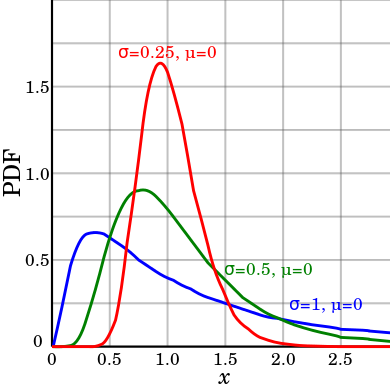
\includegraphics[width=1.5in]{./images/log-normal-dist.png}  \hfill \\
 
\subsubsection{Pareto distribution} 
Named after the economist Vilfredo Pareto, who used it to describe the distribution of wealth. \hfill \\
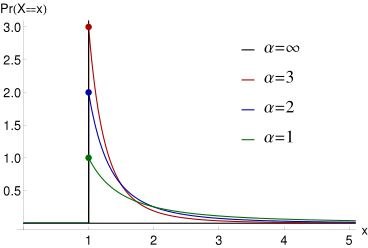
\includegraphics[width=1.5in]{./images/pareto-dist.png}  \hfill \\
Pareto distributions are often the result of generative processes with positive feedback

\subsection{Kernel density estimation}
A way to estimate the probability density function (PDF) of a random variable from a sample, in a non-parametric way.
\href{https://docs.scipy.org/doc/scipy/reference/generated/scipy.stats.gaussian_kde.html}{Scipy} has an implementation that automatically selects the kernel bandwidth. 
You can then get a non-parametric PDF, or use the method that samples from it. 

\subsection{Correlation}

\subsubsection{Pearson correlation}
$\displaystyle \rho = \frac{Cov(X,Y)}{S_X S_Y}$
Nicer to report than covariances, because its dimensionless, and the range is [-1, 1].
Works well if the relationship between variables is linear and if the variables are roughly normal.

\subsubsection{Spearman�s rank correlation}
Want more robustness in the presence of outliers?  Try Spearman's rank correlation.
To compute: compute the rank of each value, then compute Pearson�s correlation for the ranks. 
Can give higher correlations when the relationship is nonlinear or the distributions are skewed.  

\section{Biased \& unbiased estimators}
Variance is a biased estimator: when you have a sample that is small, you will under-estimate the variance of the underlying distribution. 
Amazingly, an unbiased estimator for variance: $s^2 = \frac{1}{n} (x_i - \bar{x})^2$ is  $s^2 = \frac{1}{(n - 1)} (x_i - \bar{x})^2$ 
The sample mean is unbiased. 

\section{Summarizing sample distributions}

Always keep in mind that the sampling distribution does not account for other sources of error, 
	notably sampling bias and measurement error.

After you parameterize a distribution, how do you report it? 
\begin{itemize}
	\item \textbf{Standard error} (SE) = $\sigma/\sqrt{n}$ is a measure of how far we expect the estimate to be off, on average. 
		For each simulated experiment, we compute the error, $\bar{x} ? ?$, 
			and then compute the root mean squared error (RMSE). 
		Note: as sample size increases, standard error gets smaller; standard deviation does not.
	\item \textbf{Confidence interval} (CI): a range that includes a given fraction of the sampling distribution. 
\end{itemize}
	
\subsubsection{SD vs SE}
\begin{itemize}
	\item The SD (standard deviation) quantifies scatter � how much the values vary from one another.
	\item The SEM (standard error of the mean) quantifies how precisely you know the true mean of the population. 
		It takes into account both the value of the SD and the sample size.
	\item Both SD and SEM are in the same units -- the units of the data.
	\item The SEM, by definition, is always smaller than the SD.
	\item The SEM gets smaller as your samples get larger. 
	\item The SD does not change predictably as you acquire more data. 
\end{itemize}

People often think that there is a 90\% probability that the actual parameter, $\mu$, falls in the 90\% confidence interval. 
Sadly, that is not true. 
If you want to make a claim like that, you have to use Bayesian methods


\section{Hypothesis testing}
Is the effect you see in a sample likely to appear in a larger population? 
There are several ways we could formulate this question, including Fisher null hypothesis testing, Neyman-Pearson decision theory, and Bayesian inference.
The logic of this process is similar to a proof by contradiction.

Steps:
\begin{enumerate}
	\item choose a test statistic, e.g. the difference between means of two groups. 
	\item define a null hypothesis
	\item compute a p-value, which is the probability of seeing the apparent effect if the null hypothesis is true. 
	\item interpret the result. If the p-value is low, the effect is said to be statistically significant, 
		which means that it is unlikely to have occurred by chance. 
		In that case we infer that the effect is more likely to appear in the larger population.
\end{enumerate}

Interpret p-values according to their order of magnitude.  If the p-value is
\begin{itemize}
	\item  $<$ 1\%, the effect is unlikely to be due to chance; 
	\item $>$ 10\%, the effect can plausibly be explained by chance. 
	\item P-values between 1\% and 10\% should be considered borderline.
\end{itemize}

In general the p-value for a one-sided test is about half the p-value for a two-sided test, depending on the shape of the distribution.

\subsubsection{testing a correlation}
If x and y appear correlated, mix up the x, y pairs and look at the correlation of this permuted data. 
Repeat 100x, and look at the distribution of correlations seen; 
	this gives perspective on whether the correlation is real. 
	
\subsubsection{testing proportions}
E.g. testing whether a die is fair. 
Define a test statistic to be the $\sum$ abs((actual counts) - (expected counts)).
Simulate what this test statistic ends up being for a fair die.
The p-value is the fraction of the time this statistic is at your threshold or higher. 

If instead you use the square, $\sum$ ((actual counts) - (expected counts))$^2$, large outliers are weighted more strongly, and the probability appears more extreme. 
You are now in the realm of Chi-squared tests.

\subsubsection{Chi-squared tests}
$\displaystyle \chi^2 = \sum_i \frac{(O_i - E_i)^2}{E_i}$
$O_i$ are observed frequencies, $E_i$ are expected frequencies. 


\input{./tex/experimental_design.tex}

\section{Bayesian Thinking}
Bayesian thinking is the process of updating beliefs as additional data is collected, and it's the engine behind many machine learning models.
Key concepts include conditional probability, priors and posteriors, and maximum likelihood.

\subsection{Priors and posteriors}

\subsection{Maximum likelihood}

\section{Glossary}
\smallskip \hrule height 2pt \smallskip
 
 \begin{itemize}
 	\item \textbf{complementary CDF} (CCDF, or survival function) - can ask how often the random variable is above a particular level.
		Has applications in statistical hypothesis testing, for example, because the one-sided p-value 
			is the probability of observing a test statistic at least as extreme as the one observed.
 	\item \textbf{confidence interval} - An interval that represents the expected range of an estimator if 
		an experiment is repeated many times.
	\item \textbf{effect size} - any statistic that quantitatively measures the strength of a phenomenon.
	\item \textbf{jitter} - random noise added to data for purposes of visualization.  
 	\item \textbf{oversampling} - The technique of increasing the representation of a sub-population in order to avoid errors due to small sample sizes.  
	\item \textbf{p-value} - the \underline{\textbf{p}}robability that, using a given statistical model, the statistical summary 
		(such as the sample mean difference between two compared groups) would be the same as or more extreme 
		than the actual observed results
	\item \textbf{percentile rank} - The percentage of values in a distribution that are less than or equal to a given value.
	\item \textbf{quantizing} - The opposite of smoothing is discretizing, or quantizing.
	\item \textbf{rank} The index where an element appears in a sorted list.
	\item \textbf{raw moment} - A statistic based on the sum of data raised to a power.
		E.g. the correlation between two variables, the regression coefficient in a regression, the mean difference, ...
	\item \textbf{standard error}: - The RMSE of an estimate, which quantifies variability due to sampling error 
		(but not other sources of error).
	\item \textbf{standard score} A value that has been standardized so that it is expressed in standard deviations from the mean.

 \end{itemize}


%probability distributions, 
%statistical significance, 
%hypothesis testing, and 
%regression.

%Bayesian thinking. Bayesian thinking is the process of updating beliefs as additional data is collected, and it's the engine behind many machine learning models.

%Key concepts include conditional probability, priors and posteriors, and maximum likelihood.



% Reference:  \includegraphics[width=2.5in]{figures/example_kernel_separation.pdf}  \hfill \\



\vspace{4in}
\bigskip


\end{multicols*}
\end{document}
